\documentclass[11pt,a4paper]{article}

% ---------- Paquetes ----------
\usepackage[utf8]{inputenc}
\usepackage[T1]{fontenc}
\usepackage{lmodern}
\usepackage[spanish,es-tabla,es-nodecimaldot]{babel}
\usepackage[margin=2.5cm]{geometry}
\usepackage{booktabs}
\usepackage{array}
\usepackage{caption}
\usepackage{enumitem}
\usepackage{xcolor}
\usepackage{titlesec}
\usepackage{fancyhdr}
\usepackage{graphicx}
\usepackage{float}
\usepackage[colorlinks=true,linkcolor=black,citecolor=black,urlcolor=blue!50!black]{hyperref}
\newcommand{\var}[1]{\texttt{#1}}

\setlength{\parskip}{0.45em}
\setlength{\parindent}{0pt}
\setlength{\emergencystretch}{2em}
\captionsetup{font=small,labelfont=bf}
\renewcommand{\tablename}{Tabla}
\renewcommand{\arraystretch}{1.05}
\graphicspath{{../figures/}}

\titleformat{\section}{\normalfont\Large\bfseries}{\thesection.}{0.6em}{}
\titleformat{\subsection}{\normalfont\large\bfseries}{\thesubsection}{0.6em}{}
\titlespacing*{\section}{0pt}{1.1em}{0.5em}

\pagestyle{fancy}
\fancyhf{}
\fancyhead[L]{\small Machine Learning II --- Proyecto Integrador}
\fancyhead[R]{\small Entrega Final}
\fancyfoot[C]{\small\thepage}
\renewcommand{\headrulewidth}{0.4pt}

% ---------- Datos del proyecto ----------
\newcommand{\tituloProyecto}{Predicción de deserción estudiantil en el Tecnológico de Monterrey mediante modelado avanzado de Machine Learning}
\newcommand{\nombreCurso}{Machine Learning II}
\newcommand{\nombreProfesor}{Wilmer Pineda}
\newcommand{\repo}{\url{https://github.com/miguel-camargo611/ML2-desercion-estudiantil}}
\newcommand{\repoapp}{\url{https://github.com/miguel-camargo611/desercion-app}}
\newcommand{\appurl}{\url{https://desercion-tec.streamlit.app}}

\begin{document}

% ================= PORTADA =================
\begin{titlepage}
\centering
\vspace*{1.5cm}
{\Large\bfseries Universidad Externado de Colombia\par}
\vspace{0.2cm}
{\large Departamento de Matemáticas\par}
\vspace{0.15cm}
{\large \nombreCurso\par}
\vspace{2.2cm}

{\large\scshape Proyecto Integrador --- Entrega Final\par}
\vspace{0.2cm}
{\normalsize Fase 3: consolidación, despliegue y comunicación\par}
\vspace{0.4cm}
\rule{0.6\linewidth}{0.4pt}
\vspace{0.6cm}

{\Huge\bfseries \tituloProyecto \par}
\vspace{0.6cm}
\rule{0.6\linewidth}{0.4pt}

\vfill

\begin{minipage}{0.75\linewidth}
\centering
\textbf{Integrantes}\\[0.3cm]
Miguel Camargo \\
Camilo Hernández
\end{minipage}

\vspace{1.2cm}
\textbf{Profesor:} \nombreProfesor

\vspace{1.2cm}
{\large 11 de noviembre de 2026 \par}
\vfill
\end{titlepage}

\pagenumbering{arabic}
\setcounter{page}{1}

% ================= 1. RECOMENDACIÓN =================
\section{Recomendación}

Al terminar el primer semestre, una universidad quiere saber a cuáles de sus estudiantes acompañar para que no abandonen antes de terminar el primer año. En las dos fases anteriores comparamos nueve modelos sobre 24.251 estudiantes del Tecnológico de Monterrey. En esta fase elegimos el modelo final, lo evaluamos una sola vez con datos que nunca había visto, lo pusimos a disposición en una aplicación web y lo interpretamos.

La recomendación es \textbf{ordenar a los estudiantes por su riesgo estimado y repartir el acompañamiento en tres niveles} (Tabla~\ref{tab:niveles}). Las cifras salen del conjunto de prueba sellado: 4.843 estudiantes que no se usaron para entrenar el modelo ni para tomar ninguna decisión.

\begin{table}[H]
\centering
\small
\caption{Niveles de riesgo en el conjunto de prueba. El riesgo alto agrupa al 20\,\% de estudiantes con mayor probabilidad estimada; el medio, a quienes superan el umbral validado sin estar en ese 20\,\%.}
\label{tab:niveles}
\begin{tabular}{l>{\raggedright\arraybackslash}p{2.2cm}ccc>{\raggedright\arraybackslash}p{2.9cm}}
\toprule
Nivel & Quiénes & Estudiantes & Deserción & \shortstack{Desertores\\que concentra} & Acción \\
\midrule
Alto & 20\,\% de mayor riesgo & 20\,\% & \textbf{18,2\,\%} & \textbf{48,5\,\%} & Contactar esta semana \\
Medio & Superan el umbral & 16\,\% & 7,3\,\% & 15,5\,\% & Seguimiento en el mes \\
Bajo & El resto & 64\,\% & 4,3\,\% & 36,0\,\% & Acompañamiento habitual \\
\bottomrule
\end{tabular}
\end{table}

En la práctica, de cada 100 estudiantes 20 quedan en riesgo alto, y ahí está casi la mitad de los que van a desertar. En ese grupo deserta el 18\,\%, cuatro veces más que en el nivel bajo. Si los recursos alcanzan para atender también el nivel medio, se cubre al 36\,\% de los estudiantes y se llega a 64 de cada 100 desertores.

Dos advertencias. La alerta \emph{prioriza}, no diagnostica: solo 1 de cada 7 alertados termina desertando. Por eso la acción debe ser un acompañamiento de bajo costo (una conversación, una tutoría) y nunca una sanción. Además, el modelo casi no detecta a los becarios por talento académico que abandonan, así que ese grupo necesita otra vía de seguimiento (Sección~3).

% ================= 2. MODELO FINAL =================
\section{Modelo final y reproducción del método}

\textbf{El problema.} Siguiendo a Villar y Andrade (2024), predecimos la deserción combinando lo que se sabe del estudiante al ingresar con su desempeño en el primer semestre. La variable objetivo vale 1 si el estudiante ya no está matriculado al cerrar su primer año, y solo el 7,7\,\% deserta. Con tan pocos positivos, la exactitud engaña: un modelo que diga ``nadie deserta'' acierta el 92\,\% de las veces. Por eso comparamos los modelos con el PR-AUC, que mide qué tan bien se encuentra a los desertores. El umbral de alerta se fijó con F2, que da al recall el doble de peso: dejar pasar a un estudiante que se va cuesta más que una conversación de más.

\textbf{Por qué LightGBM.} En la Segunda entrega, los cuatro modelos de \textit{boosting} quedaron empatados (PR-AUC entre 0,245 y 0,248). Elegimos entre ellos mirando cuatro frentes, como se haría antes de adoptar el modelo en una universidad:
\begin{itemize}[leftmargin=1.3em,itemsep=1pt,topsep=2pt]
\item \textbf{Desempeño.} LightGBM (0,247) no se distingue de CatBoost, XGBoost ni Gradient Boosting: con la prueba t corregida de Nadeau y Bengio, $p \geq 0{,}68$ en las tres comparaciones. Sí supera a la regresión logística ($p = 0{,}035$), el modelo de referencia del curso anterior.
\item \textbf{Estabilidad.} Su desviación entre las cinco rondas de validación (0,023) es igual a la de CatBoost.
\item \textbf{Costo.} Se entrena en 0,55 segundos, frente a los 16 de CatBoost, y su búsqueda de hiperparámetros tomó 5,5 minutos en lugar de 29,7. Con un desempeño empatado, el costo desempata.
\item \textbf{Interpretabilidad.} La regresión logística sería la más fácil de explicar, porque sus coeficientes se leen directamente, pero rinde significativamente menos. LightGBM no obliga a renunciar a la explicación: como modelo de árboles admite SHAP exacto (\textit{TreeExplainer}), que la aplicación calcula al instante para cada estudiante.
\end{itemize}

\textbf{Tres pruebas antes de abrir el conjunto de prueba.} Una revisión crítica señaló tres posibles debilidades del diseño, y las pusimos a prueba con el conjunto de desarrollo, sin tocar el de prueba (Tabla~\ref{tab:sensibilidad}).
\begin{itemize}[leftmargin=1.3em,itemsep=1pt,topsep=2pt]
\item \textbf{La rúbrica de admisión.} Falta en el 45\,\% de la cohorte AD19 y nunca en AD20, así que la columna que marca ``sin dato'' podía estar funcionando como un indicador de cohorte. No era así: quitarla no cambia el desempeño. La quitamos de todos modos, porque en una cohorte nueva la rúbrica siempre está y esa columna sería una constante.
\item \textbf{Una cohorte que el modelo no ha visto.} La validación mezclaba AD19 y AD20, pero en la práctica se entrena con el pasado y se predice el futuro. Entrenando solo con AD19 y prediciendo AD20, el PR-AUC baja de 0,220 a 0,186, aunque el modelo sigue siendo 2,8 veces mejor que el azar. Esa caída no se puede atribuir solo al cambio de cohorte, porque al entrenar con AD19 también se usa la mitad de los datos.
\item \textbf{La calibración.} Las probabilidades significan lo que dicen: en promedio, el modelo estima un 7,7\,\% de deserción y la tasa real es 7,8\,\%. Por eso la aplicación puede mostrarlas tal cual.
\end{itemize}

\begin{table}[H]
\centering
\small
\caption{Pruebas de robustez del modelo final, todas sobre el conjunto de desarrollo.}
\label{tab:sensibilidad}
\begin{tabular}{>{\raggedright\arraybackslash}p{4.3cm}>{\raggedright\arraybackslash}p{6.1cm}>{\raggedright\arraybackslash}p{4.1cm}}
\toprule
Pregunta & Resultado & Decisión \\
\midrule
\textquestiondown{}La marca ``sin dato'' de la rúbrica es un indicador de cohorte? & PR-AUC 0,2468 con la marca, 0,2467 sin ella y 0,2474 con la cohorte explícita & Se quita la marca \\
\textquestiondown{}Generaliza a una cohorte no vista? & AD19\,$\rightarrow$\,AD20: PR-AUC 0,186 frente a 0,220 mezclando cohortes; ROC-AUC 0,680 frente a 0,701 & Se reporta como limitación \\
\textquestiondown{}Las probabilidades están calibradas? & 7,73\,\% estimado frente a 7,75\,\% observado; pendiente de calibración 1,04 (ideal: 1) & Se muestran sin recalibrar \\
\bottomrule
\end{tabular}
\end{table}

\textbf{Configuración definitiva.} El flujo final es un único \textit{Pipeline} que se ajusta con el conjunto de desarrollo completo. Rellena los faltantes con la mediana, agregando una columna que marca el dato faltante salvo en la rúbrica. Estandariza las numéricas y codifica las categóricas (las de menos de 30 registros se agrupan). Los hiperparámetros salieron de la misma rejilla y la misma validación interna de la Segunda entrega: 400 árboles de 8 hojas, tasa de aprendizaje 0,02 y al menos 100 estudiantes por hoja. SMOTE volvió a quedar descartado. El umbral de alerta (0,072) se eligió con F2 sobre predicciones fuera de pliegue del conjunto de desarrollo. El modelo usa 23 variables.

\textbf{Evaluación única en prueba.} Los resultados en prueba coinciden con los de la validación cruzada (Tabla~\ref{tab:prueba}). El PR-AUC es algo menor (0,220), pero el de la validación cruzada queda dentro de su intervalo de confianza. La captura de desertores (48,5\,\%) y el recall (0,64) se mantienen. Separando por cohorte, AD20 es más difícil que AD19 (PR-AUC de 0,17 frente a 0,26): coincide con la prueba temporal y con que en AD20 desertan menos estudiantes (6,7\,\% frente a 8,5\,\%).

\begin{table}[H]
\centering
\small
\caption{Modelo final: conjunto de prueba sellado (4.843 estudiantes, 367 desertores; intervalos bootstrap al 95\,\%) frente a la validación cruzada anidada en desarrollo (media $\pm$ desviación en cinco rondas).}
\label{tab:prueba}
\begin{tabular}{lcc}
\toprule
Métrica & Prueba sellada & Validación cruzada \\
\midrule
PR-AUC (azar = 0,076) & 0,220 \; [0,183 -- 0,265] & 0,247 $\pm$ 0,023 \\
ROC-AUC & 0,708 \; [0,677 -- 0,737] & 0,716 \\
Recall con el umbral F2 & 0,64 \; [0,59 -- 0,69] & 0,67 \\
Precisión con el umbral F2 & 0,13 \; [0,12 -- 0,15] & 0,13 \\
Desertores en el 20\,\% de mayor riesgo & 48,5\,\% \; [43,6 -- 53,1] & 46,4\,\% \\
\bottomrule
\end{tabular}
\end{table}

\textbf{Contraste con el artículo.} El objetivo de Villar y Andrade es identificar a tiempo a quién apoyar. Ese objetivo se cumple aquí y, además, se adelanta: predecimos con un semestre de notas, no con dos. El núcleo del método se reprodujo (Tabla~\ref{tab:articulo}): la familia de \textit{boosting} vuelve a ganar y el desempeño académico reciente vuelve a ser la variable más importante. La diferencia está en la magnitud. Villar y Andrade reportan un F1 de hasta 0,88 en la clase desertora, y nosotros obtenemos 0,22. En la Segunda entrega mostramos que buena parte de esa distancia viene del protocolo: aplicar SMOTE antes de separar los datos, como hace el artículo, infla el F1 de nuestro modelo de 0,12 a 0,95. El resto se explica por el problema: nuestra tasa de deserción es la cuarta parte de la suya (7,7\,\% frente a 32\,\%), y predecimos con un solo semestre de notas, no con dos.

\begin{table}[H]
\centering
\small
\caption{Qué se reprodujo y qué cambió respecto a Villar y Andrade (2024).}
\label{tab:articulo}
\begin{tabular}{>{\raggedright\arraybackslash}p{2.8cm}>{\raggedright\arraybackslash}p{5.5cm}>{\raggedright\arraybackslash}p{6.2cm}}
\toprule
Aspecto & Artículo & Este proyecto \\
\midrule
Datos & Portugal: 4.424 estudiantes, tres desenlaces, 32\,\% de desertores & México: 24.251 estudiantes, dos desenlaces, 7,7\,\% de desertores \\
Información usada & Notas del 1.\textsuperscript{er} y 2.\textsuperscript{o} semestre & Solo notas del 1.\textsuperscript{er} semestre: se predice antes \\
Desbalance & SMOTE antes de separar (fuga de información) & SMOTE dentro del \textit{Pipeline}, como hiperparámetro: la validación lo descartó \\
Ajuste y validación & Optuna; prueba t sin corrección & GridSearchCV en validación cruzada anidada; prueba t corregida de Nadeau y Bengio \\
Mejor modelo & CatBoost y LightGBM & Boosting empatado; LightGBM por costo \\
Variable clave & Materias aprobadas en el 2.\textsuperscript{o} semestre & Promedio del 1.\textsuperscript{er} semestre \\
\bottomrule
\end{tabular}
\end{table}

% ================= 3. INTERPRETACIÓN =================
\section{Interpretación de los resultados}

\textbf{Qué mira el modelo.} La Figura~\ref{fig:shap} resume, con SHAP, cuánto pesa cada variable en las predicciones del conjunto de prueba y en qué dirección. Dos factores dominan, con un peso que dobla al tercero: el \textbf{promedio del primer semestre} (a mejor promedio, menos riesgo) y el \textbf{porcentaje de beca} (a más beca, menos riesgo). Les siguen el promedio de bachillerato y tres variables de contexto: la región del campus, la escuela y la educación del padre. La edad empuja en sentido contrario: los estudiantes mayores tienen más riesgo. En lenguaje institucional, el riesgo se concentra en quienes tuvieron un mal arranque académico y no tienen apoyo económico. SHAP describe cómo decide el modelo, no causas: no dice que dar más beca evite la deserción. Por ejemplo, las becas suelen exigir un promedio mínimo, así que también reflejan quién entra con buen desempeño.

\begin{figure}[H]
\centering
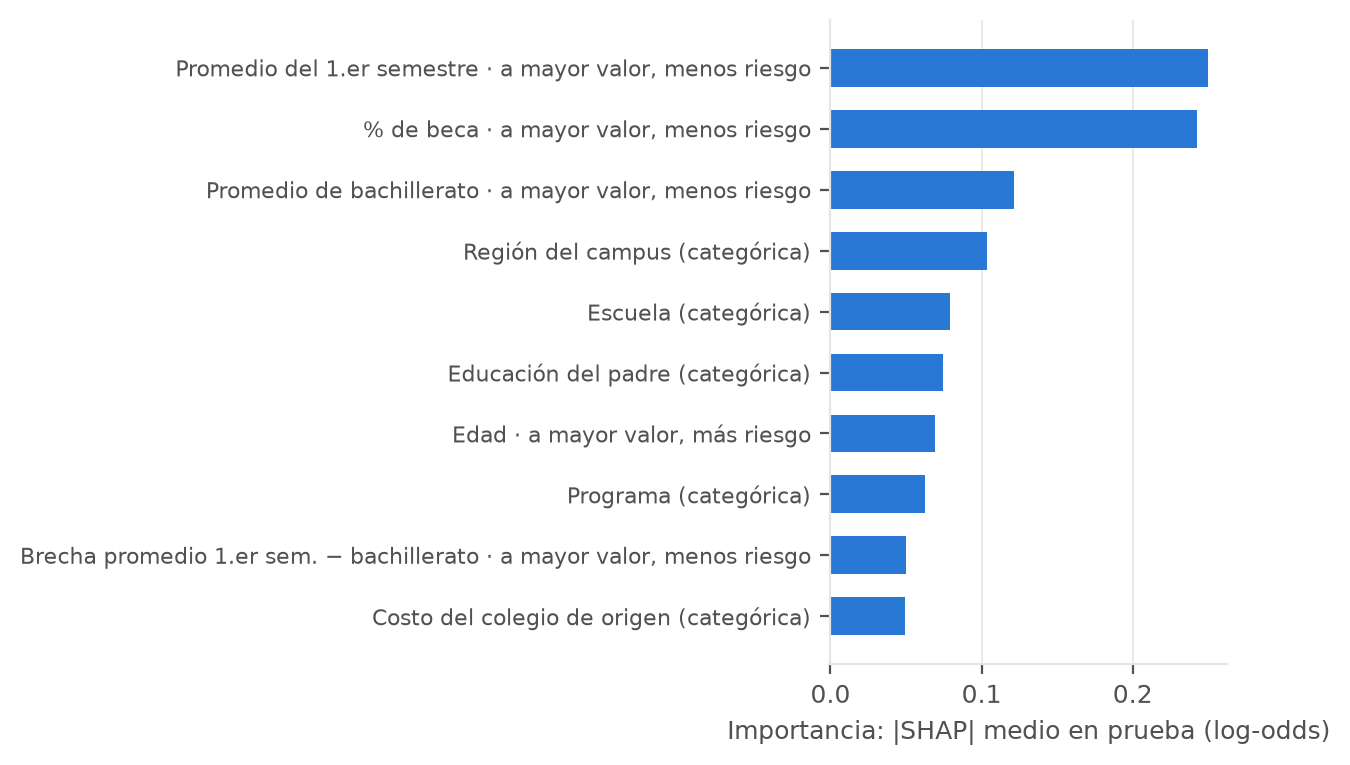
\includegraphics[width=0.78\linewidth]{fig10_shap_final.png}
\caption{Variables más influyentes del modelo final en el conjunto de prueba (media del valor absoluto de SHAP, sumando las columnas de cada variable categórica). En las numéricas se indica la dirección, según la correlación entre el valor de la variable y su aporte.}
\label{fig:shap}
\end{figure}

\textbf{Qué tan confiable es el orden y la probabilidad.} La Figura~\ref{fig:prueba}a muestra la utilidad práctica del modelo. Alertar al azar al 20\,\% de los estudiantes encontraría al 20\,\% de los desertores, mientras que siguiendo el orden del modelo se encuentra al 49\,\%. La Figura~\ref{fig:prueba}b confirma con los datos de prueba que las probabilidades están calibradas: en cada decil de riesgo, la deserción observada cae sobre la diagonal, dentro de su intervalo de confianza. Una probabilidad de 25\,\% se puede leer literalmente como ``uno de cada cuatro estudiantes así desertó''.

\begin{figure}[H]
\centering
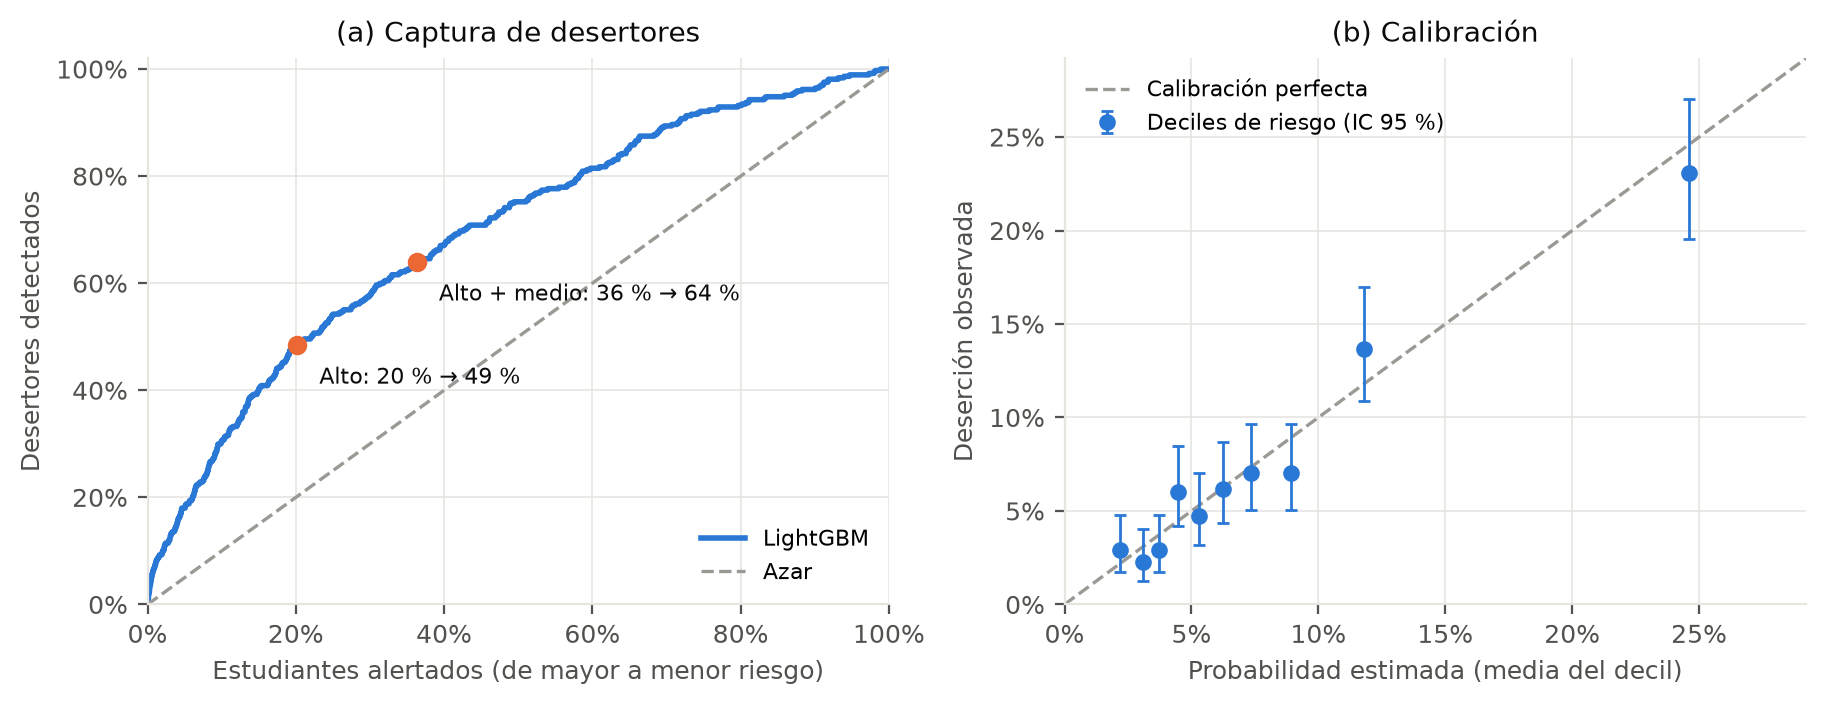
\includegraphics[width=0.95\linewidth]{fig09_prueba_final.png}
\caption{Conjunto de prueba sellado. (a) Porcentaje de desertores detectados según el porcentaje de estudiantes alertados, de mayor a menor riesgo; los puntos marcan los niveles de la Tabla~\ref{tab:niveles}. (b) Probabilidad estimada frente a deserción observada, por decil de riesgo.}
\label{fig:prueba}
\end{figure}

\textbf{Tipos de error y sus implicaciones.} De los 367 desertores del conjunto de prueba, el modelo alertó a 235 y dejó pasar a 132. A cambio emitió 1.523 falsas alarmas, unas 7,5 alertas por cada desertor encontrado. Los dos errores no cuestan lo mismo. Una falsa alarma cuesta una conversación con un estudiante que no lo necesitaba, siempre que se presente como apoyo y no como sospecha. Un desertor no detectado es un estudiante que la universidad pierde sin haber intentado nada. Por eso elegimos el umbral con F2. Si los recursos son escasos, el nivel alto por sí solo baja la carga a 5,5 alertas por desertor encontrado.

\textbf{Dónde falla.} Los errores no se reparten igual entre grupos. Entre los becarios por talento académico, el modelo detecta solo a 6 de sus 23 desertores (26\,\%), porque su beca y su buen promedio lo llevan a estimar un riesgo bajo. Entre los estudiantes sin beca, en cambio, detecta al 78\,\%, pero alerta al 57\,\% del grupo. El recall también cambia según la región: es del 46\,\% en Monterrey y del 73\,\% en Ciudad de México. La implicación es concreta: el modelo no debe ser el único filtro. Hay perfiles, como el del becario que abandona, cuyas razones no aparecen en estas variables y que requieren el criterio de los consejeros.

\textbf{Alcance de las conclusiones.} Lo anterior vale para estudiantes de pregrado del Tecnológico de Monterrey al terminar su primer semestre, con datos de las cohortes 2019 y 2020. Las relaciones que muestra SHAP son asociaciones que el modelo aprendió, no efectos causales. Llevar el modelo a otra universidad, o a otro momento de la carrera, exigiría volver a validarlo con datos de ese contexto.

% ================= 4. DESPLIEGUE =================
\section{Despliegue}

El modelo está disponible en una aplicación Streamlit pública (Figura~\ref{fig:app}; enlace en el anexo). La aplicación evalúa a un estudiante con un formulario o a muchos con un archivo CSV o Excel. Para cada uno devuelve la probabilidad, el nivel de riesgo, la acción sugerida y la explicación SHAP de esa predicción en particular. Para un grupo muestra además cuántos estudiantes hay en cada nivel, la distribución del riesgo, una lista ordenada de mayor a menor riesgo y las variables que más pesan en ese grupo.

\begin{figure}[H]
\centering
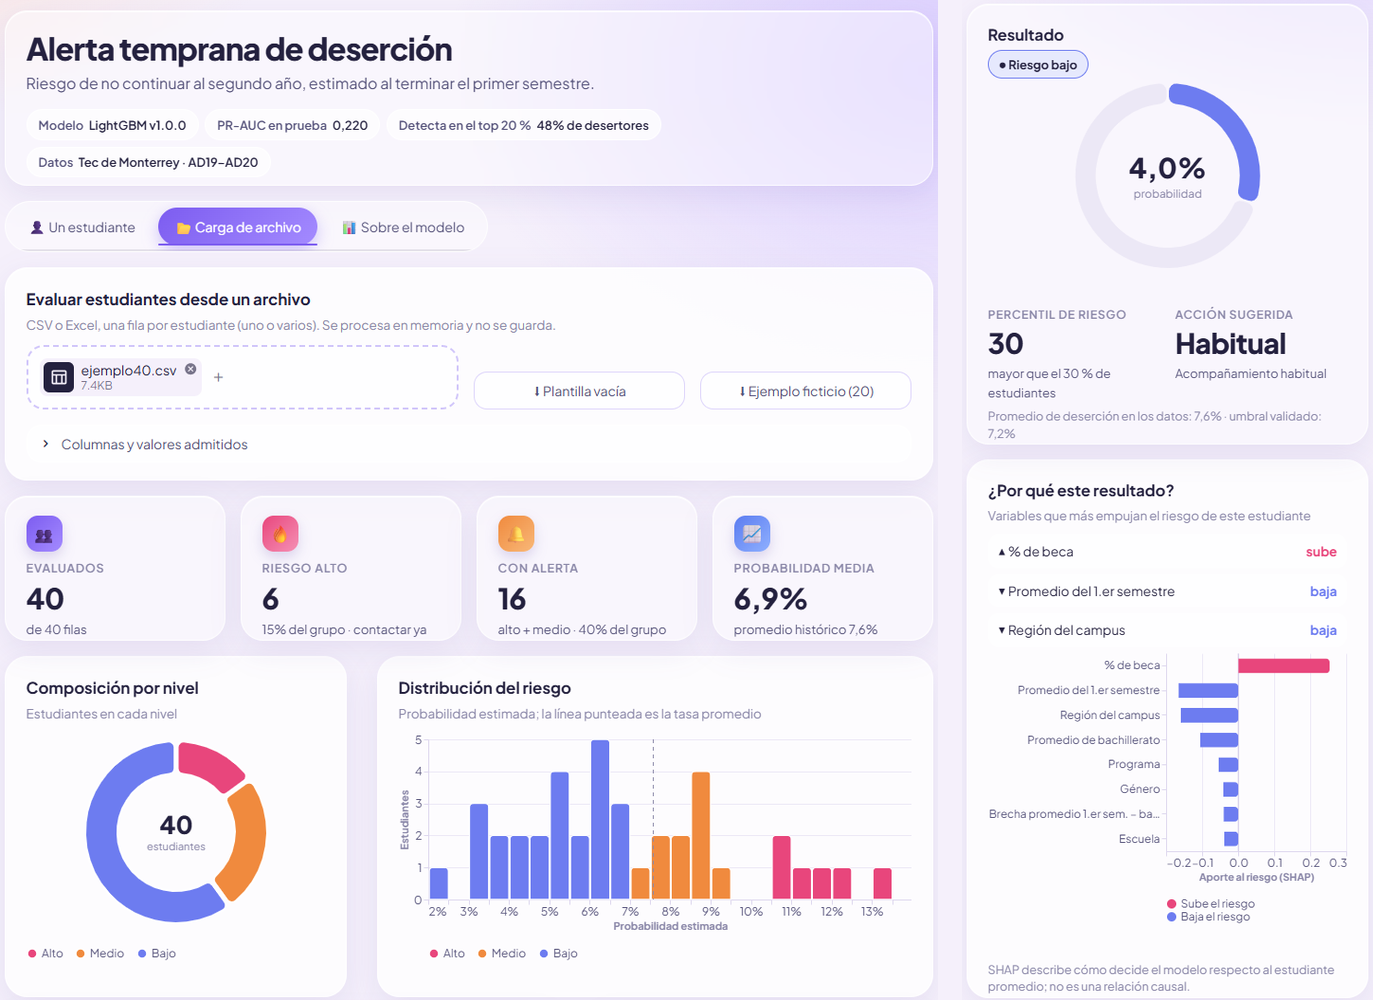
\includegraphics[width=\linewidth]{fig11_app.png}
\caption{La aplicación desplegada. Izquierda: evaluación de un archivo con 40 estudiantes ficticios. Derecha: resultado y explicación de un estudiante.}
\label{fig:app}
\end{figure}

\textbf{Coherencia entre entrenamiento y uso.} La aplicación no vuelve a implementar el preprocesamiento: carga el mismo \textit{Pipeline} serializado que se evaluó en prueba, con las mismas versiones de las librerías. Lo acompaña un contrato que fija el orden de las variables, los rangos y las categorías vistos en el entrenamiento, el umbral y la versión del modelo. Una entrada fuera de rango o con una categoría desconocida no se predice: se informa cuál es el error. El único cálculo propio de la aplicación es la variable construida (promedio del primer semestre menos promedio de bachillerato), que repite la fórmula del entrenamiento y está cubierta por una prueba automática. Para comprobar que el modelo da lo mismo en cualquier entorno guardamos un perfil \emph{ficticio} con su probabilidad. Esa predicción de referencia coincide hasta la sexta cifra decimal en el computador de desarrollo, dentro de un contenedor Docker y en un entorno limpio igual al de Streamlit Cloud.

\textbf{Reproducibilidad.} Además de Streamlit Cloud, el despliegue se puede reconstruir con Docker Compose, siguiendo el laboratorio de clase: el contenedor corre sin privilegios de administrador, tiene chequeo de salud y queda detrás de un proxy con HTTPS, sin exponer el puerto interno. Doce pruebas automáticas verifican el contrato, la paridad y la validación de entradas, y corren en cada actualización del repositorio. La aplicación se publica desde un repositorio público que solo contiene la aplicación y el modelo, sin datos de estudiantes. El repositorio principal sigue siendo privado, porque los datos del TEC DataHub no se pueden redistribuir.

% ================= 5. LIMITACIONES =================
\section{Calidad, limitaciones y proyección}

\textbf{Limitaciones.}
\begin{enumerate}[leftmargin=1.5em,itemsep=1pt,topsep=2pt]
\item \textbf{Datos.} Los datos son reales, de modo que no hubo supuestos de simulación, pero solo dos cohortes registran las notas del primer semestre. Además, la pandemia afectó a ambas: el segundo semestre de AD19 y todo el primer año de AD20. El nivel socioeconómico no se pudo usar porque falta en la mitad de los estudiantes, así que el modelo solo ve la situación económica a través de la beca y del costo del colegio de origen.
\item \textbf{Generalización.} En una cohorte nueva conviene esperar un desempeño algo menor que el de la validación cruzada (PR-AUC cercano a 0,19 en la prueba temporal) y un nivel de probabilidades corrido: en AD20, el modelo entrenado con AD19 estimó 7,9\,\% de deserción, y la real fue 6,7\,\%.
\item \textbf{Señal moderada.} Con un ROC-AUC de 0,71, el modelo sirve para priorizar, no para decidir sobre un estudiante concreto.
\item \textbf{Sesgo hacia quien no tiene beca.} Como se vio en la Sección~3, el riesgo estimado se concentra en los estudiantes sin beca, y los becarios que abandonan pasan casi inadvertidos.
\item \textbf{Sobreajuste y estabilidad.} El riesgo de sobreajuste se controló en tres capas, y en ninguna aparecieron señales de él.
\begin{itemize}[leftmargin=1.2em,itemsep=0pt,topsep=1pt]
\item La validación cruzada anidada separa el ajuste de hiperparámetros de la estimación del desempeño.
\item La curva de validación muestra dónde empieza a memorizar: con 128 hojas el PR-AUC de entrenamiento sube a 0,91 mientras el de validación baja a 0,23. Por eso se eligieron árboles pequeños, de 8 hojas (0,25 en validación).
\item El conjunto de prueba confirma lo que anticipó la validación.
\end{itemize}
El desempeño varía poco entre rondas (desviación de 0,023). Aun así, la prueba es un único corte, y por eso reportamos intervalos de confianza (PR-AUC entre 0,18 y 0,26) y no un solo número.
\end{enumerate}

\textbf{Mejoras inmediatas.} Cada mejora responde a una de las limitaciones anteriores:
\begin{itemize}[leftmargin=1.3em,itemsep=1pt,topsep=2pt]
\item Recalibrar las probabilidades con cada cohorte nueva, porque su nivel se corre de un año a otro.
\item Sumar señales tempranas del semestre, como la asistencia o el uso de la plataforma virtual, que podrían revelar el riesgo de los becarios, hoy invisibles para el modelo.
\item Revisar el recall por grupo en cada cohorte, para que la carga de alertas no recaiga siempre sobre los mismos estudiantes.
\end{itemize}

\textbf{Proyección.} Hacia \textit{MLOps}, el siguiente paso es tratar cada cohorte nueva como un ciclo:
\begin{itemize}[leftmargin=1.3em,itemsep=1pt,topsep=2pt]
\item vigilar si cambian las entradas y la calibración, comparando la tasa estimada con la observada;
\item reentrenar validando siempre con la cohorte más reciente;
\item versionar cada modelo con su contrato. El versionado ya existe en los metadatos, y las pruebas ya corren en integración continua.
\end{itemize}
Hacia \textit{Deep Learning}, la oportunidad no está en reemplazar el \textit{boosting} con estos mismos datos tabulares, donde suele seguir siendo el más fuerte, sino en usar información que hoy no tenemos. Con las notas semestre a semestre, un modelo secuencial (redes recurrentes o \textit{transformers}) podría aprender la trayectoria del estudiante y no solo una fotografía del primer semestre.

\textbf{En resumen.} El modelo final ordena a los estudiantes de manera útil: el 20\,\% de mayor riesgo concentra la mitad de los desertores, y sus probabilidades se pueden leer literalmente. Se eligió LightGBM porque empata con los mejores y es el más barato de mantener. Su desempeño en prueba confirma lo que anticipó la validación, y su uso queda acotado por las limitaciones de esta sección: priorizar acompañamiento, recalibrar con cada cohorte y no depender solo de él para los perfiles donde falla.

% ================= BIBLIOGRAFÍA =================
\begin{thebibliography}{10}
\footnotesize
\setlength{\itemsep}{1pt}

\bibitem{alvarado2022}
Alvarado-Uribe, J., Mejía-Almada, P., Masetto Herrera, A. L., Molontay, R., Hilliger, I., Hegde, V., Montemayor Gallegos, J. E., Ramírez Díaz, R. A., \& Ceballos, H. G. (2022). Student Dataset from Tecnologico de Monterrey in Mexico to Predict Dropout in Higher Education. \textit{Data}, 7(9), 119. \url{https://doi.org/10.3390/data7090119}

\bibitem{chawla2002}
Chawla, N. V., Bowyer, K. W., Hall, L. O., \& Kegelmeyer, W. P. (2002). SMOTE: synthetic minority over-sampling technique. \textit{Journal of Artificial Intelligence Research}, 16, 321--357.

\bibitem{ke2017}
Ke, G., Meng, Q., Finley, T., Wang, T., Chen, W., Ma, W., Ye, Q., \& Liu, T.-Y. (2017). LightGBM: A highly efficient gradient boosting decision tree. \textit{Advances in Neural Information Processing Systems}, 30.

\bibitem{lemaitre2017}
Lemaître, G., Nogueira, F., \& Aridas, C. K. (2017). Imbalanced-learn: A Python toolbox to tackle the curse of imbalanced datasets in machine learning. \textit{Journal of Machine Learning Research}, 18(17), 1--5.

\bibitem{lundberg2017}
Lundberg, S. M. \& Lee, S.-I. (2017). A unified approach to interpreting model predictions. \textit{Advances in Neural Information Processing Systems}, 30.

\bibitem{nadeau2003}
Nadeau, C. \& Bengio, Y. (2003). Inference for the generalization error. \textit{Machine Learning}, 52(3), 239--281.

\bibitem{pedregosa2011}
Pedregosa, F., Varoquaux, G., Gramfort, A., Michel, V., Thirion, B., Grisel, O., et al. (2011). Scikit-learn: Machine learning in Python. \textit{Journal of Machine Learning Research}, 12, 2825--2830.

\bibitem{villar2024}
Villar, A. \& Robledo Velini de Andrade, C. (2024). Supervised machine learning algorithms for predicting student dropout and academic success: a comparative study. \textit{Discover Artificial Intelligence}, 4:2. \url{https://doi.org/10.1007/s44163-023-00079-z}

\end{thebibliography}

% ================= ANEXOS =================
\section*{Anexo A: aplicación, código y reproducibilidad}

\begin{itemize}[leftmargin=1.3em,itemsep=2pt,topsep=2pt]
\item \textbf{Aplicación desplegada:} \appurl
\item \textbf{Repositorio de la aplicación} (público, sin datos):\\ \repoapp
\item \textbf{Repositorio del proyecto} (privado; el profesor fue invitado como colaborador):\\ \repo
\end{itemize}
Para repetir todos los resultados: instalar el entorno con \texttt{pip install -e .} (versiones fijadas), copiar el Excel del TEC DataHub en \texttt{data/raw/} y ejecutar \texttt{desercion all}. Todo el flujo usa la semilla 42. El modelo final se obtiene con \texttt{desercion final}, que evalúa el conjunto de prueba y se niega a repetir esa evaluación salvo que se pida de forma explícita. Las cifras y figuras de este informe salen de \texttt{desercion final\_report}.

\textbf{Cómo ejecutar la aplicación.} No necesita los datos del TEC, porque el modelo ya entrenado viene incluido en el repositorio de la aplicación:
\begin{enumerate}[leftmargin=1.5em,itemsep=1pt,topsep=2pt]
\item \texttt{git clone https://github.com/miguel-camargo611/desercion-app.git} y entrar a la carpeta.
\item \texttt{pip install -r app/requirements.txt} (Python 3.13; versiones iguales a las del entrenamiento).
\item \texttt{streamlit run app/main.py} y abrir \texttt{http://localhost:8501}.
\end{enumerate}
Con Docker, desde la carpeta \texttt{deploy/} del repositorio del proyecto: \texttt{docker compose up -d -{}-build}. La guía completa, que incluye Streamlit Cloud, Google Cloud y las pruebas de aceptación, está en \texttt{deploy/README.md}.

\section*{Anexo B: uso de inteligencia artificial}

\textbf{Herramienta.} Claude Code (Anthropic), como apoyo para escribir código y revisar textos. No generó el trabajo de una sola vez: avanzamos por rondas, y en cada una revisamos lo propuesto antes de seguir.

\textbf{Decisiones que tomó el equipo.} Limitar el proyecto a un solo escenario, el cierre del primer semestre. Excluir las variables socioeconómicas que no eran utilizables, en lugar de rellenarlas. Elegir LightGBM por costo dentro del empate del \textit{boosting}. Ante la revisión crítica que señaló la falta de validación temporal y el posible efecto de la rúbrica, ponerla a prueba con experimentos en lugar de rehacer todo el flujo, y quitar la marca de la rúbrica después de ver que no aportaba. Desplegar en Streamlit y publicar la aplicación sin exponer el repositorio ni los datos.

\textbf{Verificaciones.} El modelo base reprodujo exactamente, pliegue por pliegue, los resultados de la Segunda entrega. Repetir la evaluación final dio cifras idénticas. Cada cambio se acompañó de pruebas automáticas. La aplicación se revisó con capturas reales del navegador y se probó en un entorno limpio igual al de Streamlit Cloud antes de publicarla.

\textbf{Riesgo detectado.} La validación cruzada mezclaba las dos cohortes, lo que podía sobrestimar el desempeño en una cohorte nueva. No lo ocultamos: lo medimos (Tabla~\ref{tab:sensibilidad}) y lo reportamos como limitación con su cifra.

\end{document}
